\section{Results}
\label{sec:results}

\subsection{Testing the Asymptotic Behaviour}

The asymptotic behaviour of an implementation of above formulas for the magnetic vector potential
and magnetic field needs to be tested before using that implementation in daily routine work.
A set of critical test points used to check this is shown in Fig.~\ref{fig:circularLoop_criticalPoints}
for the case of the circular wire loop.
\begin{figure}[htbp]
 \centering
 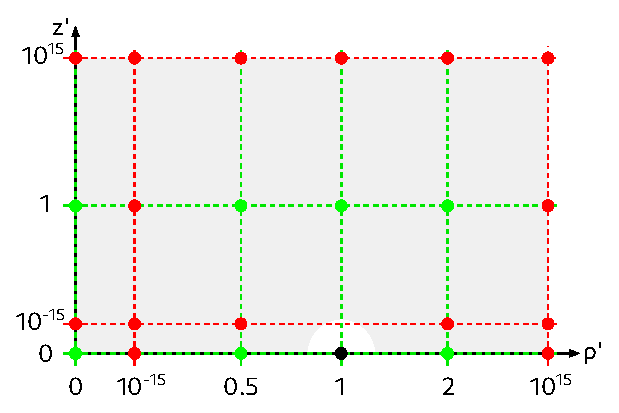
\includegraphics{img/circularLoop_criticalPoints.eps}
 \caption{Test points in the $R$-$Z$-plane for a circular wire loop (black dot).
          The axes are labelled in normalized cylindrical coordinates ($\rho' = \rho / a$, $z' = z / a$; $a$ is the radius of the wire loop).
          Green dashed lines indicate values of $\rho'$ and $z'$ which are well handled by a naive implementation.
          Green dots denote points at which a naive implementation yields satisfactory results.
          Red dashed lines indicate values of $\rho'$ and $z'$ which induce the requirement for robust asymptotic behaviour.
          Red dots denote points at which a naive implementation usually fails.
          The grey shaded area in the background indicates the region in which the reference implementation yields accurate results.
          Note that the problem is symmetric in $z$ direction, even though only the positive-$z$ quadrant is considered here.}
 \label{fig:circularLoop_criticalPoints}
\end{figure}

Reference outputs have been computed using the \texttt{mpmath} Python package~\cite{mpmath}.
The reference implementation was tested at a subset of the test points against Mathematica~\cite{Mathematica}.
The results are listed in Table~\ref{tab:ref_cylWireLoop}.
\begin{table}[htbp]
  \centering
  \begin{tabular}{c|c|c|c}
    case & $\rho'$ & $z'$ & $A_\varphi$ / Tm \\
    \hline
     0 & $0$        & $0$        & \texttt{0.0000000000000000e+00} \\
     1 & $10^{-15}$ & $0$        & \texttt{3.5499996985564660e-20} \\
     2 & $0.5$      & $0$        & \texttt{1.9733248350774467e-05} \\
     3 & $2$        & $0$        & \texttt{9.8666241753872340e-06} \\
     4 & $10^{15}$  & $0$        & \texttt{3.5499996985564664e-35} \\
     5 & $0$        & $10^{-15}$ & \texttt{0.0000000000000000e+00} \\
     6 & $10^{-15}$ & $10^{-15}$ & \texttt{3.5499996985564660e-20} \\
     7 & $0.5$      & $10^{-15}$ & \texttt{1.9733248350774467e-05} \\
     8 & $2$        & $10^{-15}$ & \texttt{9.8666241753872340e-06} \\
     9 & $10^{15}$  & $10^{-15}$ & \texttt{3.5499996985564664e-35} \\
    10 & $0$        & $1$        & \texttt{0.0000000000000000e+00} \\
    11 & $10^{-15}$ & $1$        & \texttt{1.2551144300297384e-20} \\
    12 & $0.5$      & $1$        & \texttt{5.8203906810256120e-06} \\
    13 & $1$        & $1$        & \texttt{8.8857583532073070e-06} \\
    14 & $2$        & $1$        & \texttt{6.2831799875378960e-06} \\
    15 & $10^{15}$  & $1$        & \texttt{3.5499996985564664e-35} \\
    16 & $0$        & $10^{15}$  & \texttt{0.0000000000000000e+00} \\
    17 & $10^{-15}$ & $10^{15}$  & \texttt{3.5499996985564664e-65} \\
    18 & $0.5$      & $10^{15}$  & \texttt{1.7749998492782333e-50} \\
    19 & $1$        & $10^{15}$  & \texttt{3.5499996985564666e-50} \\
    20 & $2$        & $10^{15}$  & \texttt{7.0999993971129330e-50} \\
    21 & $10^{15}$  & $10^{15}$  & \texttt{1.2551144300297385e-35}
  \end{tabular}
  \caption{Reference outputs for testing an implementation of \eqn{A_phi_final}, computed using arbirary-precision arithmetic.
           The displayed values for $A_\varphi$ are rounded to the nearest 64-bit \texttt{double} precision value (IEEE~754).
           The loop current was chosen as $I = \SI{113}{\ampere}$.}
  \label{tab:ref_cylWireLoop}
\end{table}

It turns out that most of these problems have been considered in Ref.~\cite{walstrom_2017} already.
